%% European Journal of Operational Research -- Elsevier elsarticle class.
%% Compile with: latexmk -pdf main.tex   (or: make)
\documentclass[preprint,authoryear,11pt]{elsarticle}

\usepackage{amsmath,amssymb,amsthm}
\usepackage{booktabs}
\usepackage{algorithm}
\usepackage{algpseudocode}
\usepackage{graphicx}
\graphicspath{{./}}
\usepackage{url}
\usepackage{longtable}
\usepackage{multirow}
\usepackage{array}
\newcolumntype{P}[1]{>{\raggedright\arraybackslash}p{#1}}
% Parameter and instance names are set in a monospaced face, which TeX will
% not hyphenate by default, so a long one pushes its line into the margin.
\usepackage[htt]{hyphenat}
% A table with one column per instance is naturally wide. This shrinks a
% table only when it would otherwise run into the margin, and leaves one
% that already fits at its natural size, so the type size stays uniform
% across the tables that do fit.
\newcommand{\fittable}[1]{%
  \resizebox{\ifdim\width>\linewidth\linewidth\else\width\fi}{!}{#1}}
\usepackage{tikz}
\usetikzlibrary{fit,backgrounds,arrows.meta,positioning,shapes.geometric}

\newtheorem{theorem}{Theorem}
\newtheorem{lemma}[theorem]{Lemma}
\newtheorem{corollary}[theorem]{Corollary}
\newtheorem{proposition}[theorem]{Proposition}
\theoremstyle{definition}
\newtheorem{definition}[theorem]{Definition}
\newtheorem{remark}[theorem]{Remark}

\journal{Computational Optimization and Applications}
\usepackage{xr}
\externaldocument[M-]{cascade-mis-coap}
\begin{document}
\begin{frontmatter}
\title{Supplementary material for ``Exact Large-Neighbourhood Search for the
Maximum Independent Set Problem on Massive Sparse Graphs''}
\author{Quang-Vinh Dang}
\address{British University Vietnam, Hung Yen, Vietnam. Corresponding author: vinh.dq4@buv.edu.vn}
\end{frontmatter}

\noindent\textbf{Article:} Exact Large-Neighbourhood Search for the Maximum Independent Set Problem on Massive Sparse Graphs.
\textbf{Journal:} Computational Optimization and Applications.
\textbf{Author:} Quang-Vinh Dang, British University Vietnam, vinh.dq4@buv.edu.vn.
\par\medskip

This document (Online Resource 1) holds material that supports the main manuscript but does not fit
its page limit: proofs of the standard reduction rules, the per-family result
tables, and the secondary experiments (seed study, convergence, long budget,
exact solvers, replication on a second platform), the implementation notes and the
instance appendices. Section, table and figure numbers prefixed with ``M-'' in the
source refer to the main manuscript.

\section{Proofs for the reduction rules}
\begin{lemma}[Simplicial vertices]
\label{lem:simplicial}
If $N(v)$ induces a clique then some maximum independent set contains $v$.
\end{lemma}

\begin{proof}
Let $S$ be a maximum independent set with $v \notin S$. Since $N(v)$ is a
clique, $|S \cap N(v)| \le 1$. If $S \cap N(v) = \emptyset$ then $S \cup \{v\}$
is independent and larger, contradicting maximality. Otherwise
$S \cap N(v) = \{u\}$ for a single $u$, and $(S \setminus \{u\}) \cup \{v\}$ is
independent, of the same size, and contains $v$.
\end{proof}

Degree-0 and degree-1 vertices are the special cases $|N(v)| \in \{0,1\}$.

\begin{lemma}[Domination]
\label{lem:domination}
If $uv \in E$ and $N[u] \subseteq N[v]$ then some maximum independent set
excludes $v$.
\end{lemma}

\begin{proof}
Let $S$ be a maximum independent set containing $v$. Then $u \notin S$, because
$u$ and $v$ are adjacent. Consider $S' = (S \setminus \{v\}) \cup \{u\}$. Any
neighbour of $u$ lies in $N[u] \subseteq N[v]$, that is, it is either $v$, which
has been removed, or a neighbour of $v$, which is not in $S$ because $v \in S$.
Hence $S'$ is independent, has the same size as $S$, and excludes $v$.
\end{proof}

\begin{lemma}[Degree-2 folding]
\label{lem:fold}
Let $N(v) = \{u,w\}$ with $uw \notin E$, and let $G'$ be obtained from $G$ by
deleting $v,u,w$ and adding a vertex $f$ adjacent to
$(N(u) \cup N(w)) \setminus \{v,u,w\}$. Then $\alpha(G) = \alpha(G') + 1$.
\end{lemma}

\begin{proof}
($\ge$) Let $T$ be a maximum independent set of $G'$. If $f \notin T$ then
$T \cup \{v\}$ is independent in $G$, since $v$'s only neighbours are $u$ and
$w$, neither of which is in $T$. If $f \in T$ then $(T \setminus \{f\}) \cup
\{u,w\}$ is independent in $G$: $u$ and $w$ are non-adjacent by assumption, and
any other neighbour of $u$ or $w$ is adjacent to $f$ and hence outside $T$.
Either way we obtain an independent set of size $|T| + 1$.

($\le$) Let $S$ be a maximum independent set of $G$. We first argue that $S$
may be taken to contain $v$, or to contain both $u$ and $w$. Note that
Lemma~\ref{lem:simplicial} is \emph{not} available here: its hypothesis is that
$N(v)$ induces a clique, and $N(v) = \{u,w\}$ with $uw \notin E$ is precisely the
case in which it does not. We argue directly instead. If $S$ contains neither
$u$ nor $w$, then $S \cup \{v\}$ is independent, because $u$ and $w$ are the only
neighbours of $v$; maximality of $S$ therefore forces $v \in S$ already. If $S$
contains exactly one of them, say $u$, then $(S \setminus \{u\}) \cup \{v\}$ is
independent --- the only neighbours of $v$ are $u$, which has been removed, and
$w$, which is not in $S$ --- and has the same size, so we may replace $S$ by it
and again have $v \in S$. In the one remaining case $u,w \in S$, and then
$v \notin S$ because $v$ is adjacent to both. In the first case
$S \setminus \{v\}$ is independent in $G'$ and avoids $f$. In the second,
$(S \setminus \{u,w\}) \cup \{f\}$ is independent in $G'$, because no neighbour
of $f$ other than through $u$ or $w$ exists. Either way we obtain an independent
set of $G'$ of size $|S| - 1$.
\end{proof}


\section{Per-family results}
\label{sec:s-quality}
Tables~\ref{tab:quality-geometric}--\ref{tab:quality-bhoslib} give, for each family, the size of the
independent set each solver returned at the 60\,s budget.
\begin{table}[htbp]
\centering
\caption{Geometric (Delaunay and random geometric): size of the independent set found within the 60\,s budget (larger is better). Best value per instance in bold.}
\label{tab:quality-geometric}
\small
\fittable{\begin{tabular}{lrrrrrrr}
\toprule
Instance & \textsc{Cascade} & ReduMIS & OnlineMIS & NearLinear & LinearTime & NuMVC & FastVC \\
\midrule
\texttt{rgg16} & \textbf{16086} & \textbf{16086} & 16082 & 16035 & 15321 & 15905 & 16085 \\
\texttt{del16} & \textbf{20647} & 20640 & 20630 & 20284 & 20213 & 20180 & 20638 \\
\texttt{rgg18} & \textbf{64278} & \textbf{64278} & 63912 & 64094 & 61282 & 62548 & 64242 \\
\texttt{del18} & \textbf{82656} & 82385 & 82019 & 81211 & 80881 & 80695 & 82579 \\
\texttt{rgg20} & \textbf{256994} & \textbf{256994} & 242366 & 256277 & 244769 & 239118 & 256680 \\
\texttt{del20} & \textbf{330066} & 321566 & 311146 & 324619 & 323438 & 311421 & 329802 \\
\bottomrule
\end{tabular}}
\end{table}

\begin{table}[htbp]
\centering
\caption{Road networks: size of the independent set found within the 60\,s budget (larger is better). Best value per instance in bold.}
\label{tab:quality-road}
\small
\fittable{\begin{tabular}{lrrrrrrr}
\toprule
Instance & \textsc{Cascade} & ReduMIS & OnlineMIS & NearLinear & LinearTime & NuMVC & FastVC \\
\midrule
\texttt{roadNet-PA} & 533627 & \textbf{533628} & 515876 & 531184 & 530910 & 513067 & 532571 \\
\texttt{roadNet-CA} & \textbf{961851} & \textbf{961851} & 924236 & 957199 & 956573 & 915797 & 959909 \\
\bottomrule
\end{tabular}}
\end{table}

\begin{table}[htbp]
\centering
\caption{Social networks: size of the independent set found within the 60\,s budget (larger is better). Best value per instance in bold.}
\label{tab:quality-social}
\small
\fittable{\begin{tabular}{lrrrrrrr}
\toprule
Instance & \textsc{Cascade} & ReduMIS & OnlineMIS & NearLinear & LinearTime & NuMVC & FastVC \\
\midrule
\texttt{ca-AstroPh} & \textbf{6760} & \textbf{6760} & \textbf{6760} & \textbf{6760} & 6759 & \textbf{6760} & \textbf{6760} \\
\texttt{ca-CondMat} & \textbf{9612} & \textbf{9612} & 9601 & \textbf{9612} & 9611 & 9611 & \textbf{9612} \\
\texttt{email-Enron} & \textbf{22255} & \textbf{22255} & 22227 & \textbf{22255} & \textbf{22255} & 22253 & \textbf{22255} \\
\texttt{com-dblp} & \textbf{152131} & \textbf{152131} & 152061 & \textbf{152131} & 152129 & 152112 & \textbf{152131} \\
\texttt{com-amazon} & \textbf{174632} & \textbf{174632} & 172685 & 174627 & 174612 & 174510 & 174605 \\
\texttt{com-youtube} & \textbf{857945} & \textbf{857945} & 857680 & \textbf{857945} & 857944 & 857708 & \textbf{857945} \\
\texttt{soc-pokec-relationships} & 788866 & -- & 776663 & 789161 & 789003 & 787320 & \textbf{789352} \\
\texttt{as-skitter} & 1170576 & \textbf{1170580} & 1152300 & 1170541 & 1170410 & 1168352 & 1168417 \\
\texttt{wiki-Talk} & \textbf{2338222} & \textbf{2338222} & 2338207 & \textbf{2338222} & \textbf{2338222} & 2338220 & \textbf{2338222} \\
\texttt{com-lj} & \textbf{2085626} & \textbf{2085626} & 2066610 & 2085604 & 2085353 & -- & 2085169 \\
\bottomrule
\end{tabular}}
\end{table}

\begin{table}[htbp]
\centering
\caption{Web graphs: size of the independent set found within the 60\,s budget (larger is better). Best value per instance in bold.}
\label{tab:quality-web}
\small
\fittable{\begin{tabular}{lrrrrrrr}
\toprule
Instance & \textsc{Cascade} & ReduMIS & OnlineMIS & NearLinear & LinearTime & NuMVC & FastVC \\
\midrule
\texttt{web-Stanford} & 163375 & \textbf{163390} & 162453 & 163198 & 163121 & 162453 & 162953 \\
\texttt{web-BerkStan} & 408380 & \textbf{408482} & 406062 & 408054 & 407716 & 405003 & 406323 \\
\bottomrule
\end{tabular}}
\end{table}

\begin{table}[htbp]
\centering
\caption{BHOSLIB \texttt{frb}: size of the independent set found within the 60\,s budget (larger is better). Best value per instance in bold.}
\label{tab:quality-bhoslib}
\small
\fittable{\begin{tabular}{lrrrrrrr}
\toprule
Instance & \textsc{Cascade} & ReduMIS & OnlineMIS & NearLinear & LinearTime & NuMVC & FastVC \\
\midrule
\texttt{frb30-15-1} & \textbf{30} & \textbf{30} & 29 & 24 & 22 & \textbf{30} & \textbf{30} \\
\texttt{frb35-17-1} & 34 & \textbf{35} & 33 & 27 & 25 & \textbf{35} & \textbf{35} \\
\texttt{frb40-19-1} & 39 & \textbf{40} & 39 & 27 & 29 & \textbf{40} & \textbf{40} \\
\texttt{frb45-21-1} & 43 & 43 & 42 & 33 & 32 & \textbf{45} & \textbf{45} \\
\texttt{frb50-23-1} & 48 & 49 & 48 & 35 & 33 & \textbf{50} & 49 \\
\texttt{frb53-24-1} & 50 & 51 & 49 & 38 & 40 & \textbf{52} & 51 \\
\texttt{frb59-26-1} & 56 & 57 & 56 & 43 & 43 & \textbf{58} & 56 \\
\bottomrule
\end{tabular}}
\end{table}

\begin{table}[htbp]
\centering
\caption{Where the advantage over \textsc{ReduMIS} comes from, per instance family, at the 60-second budget. \emph{Net} is the sum over the family of $|S_{\textsc{cascade}}|-|S_{\textsc{ReduMIS}}|$; higher is better. The one instance on which \textsc{ReduMIS} returned nothing within the budget is excluded from its family's counts.}
\label{tab:whence}
\fittable{
\begin{tabular}{l r r r r r}
\toprule
Family & Instances & Ahead & Tied & Behind & Net \\
\midrule
geometric & 6 & 3 & 3 & 0 & +8778 \\
road & 2 & 0 & 1 & 1 & -1 \\
web & 2 & 0 & 0 & 2 & -117 \\
social $^{*}$ & 9 & 0 & 8 & 1 & -4 \\
bhoslib & 7 & 0 & 2 & 5 & -5 \\
\midrule
\textbf{All} & 26 & 3 & 14 & 9 & +8651 \\
\bottomrule
\end{tabular}
}
\\[2pt]\footnotesize $^{*}$ one instance excluded: \textsc{ReduMIS} exceeded the budget.
\end{table}

\section{Convergence}
\label{sec:convergence}

Table~\ref{M-tab:longbudget} shows what each solver reaches by the end of its
budget; Figure~\ref{fig:convergence} shows how it gets there. Four instances
were re-run with every improvement of the incumbent recorded against the wall
clock. Only the three solvers that report improvements as they happen are
plotted; the reduction-only baselines produce a single point.

The shapes differ more than the endpoints do. On \texttt{del18} and
\texttt{roadNet-PA} our solver reaches a value the others need most of the
budget to approach, and then flattens: the kernelization and the first dive do
most of the work, and the region moves refine it. On \texttt{web-Stanford} it
converges almost immediately and improves six times in sixty seconds, which is
the same observation the long-budget run makes from the other direction --- there
is very little left to find once the graph has been reduced. The dense instance
inverts the picture. All three solvers finish on the same value of 40, but NuMVC
reaches it after $0.2$ seconds and FastVC after $0.8$, where we need $6.6$: on a
graph this dense the region move has to work its way to what a specialised local
search finds almost at once, and the tie at the deadline hides a large
difference in how quickly it was reached.

\begin{figure}[htbp]
\centering
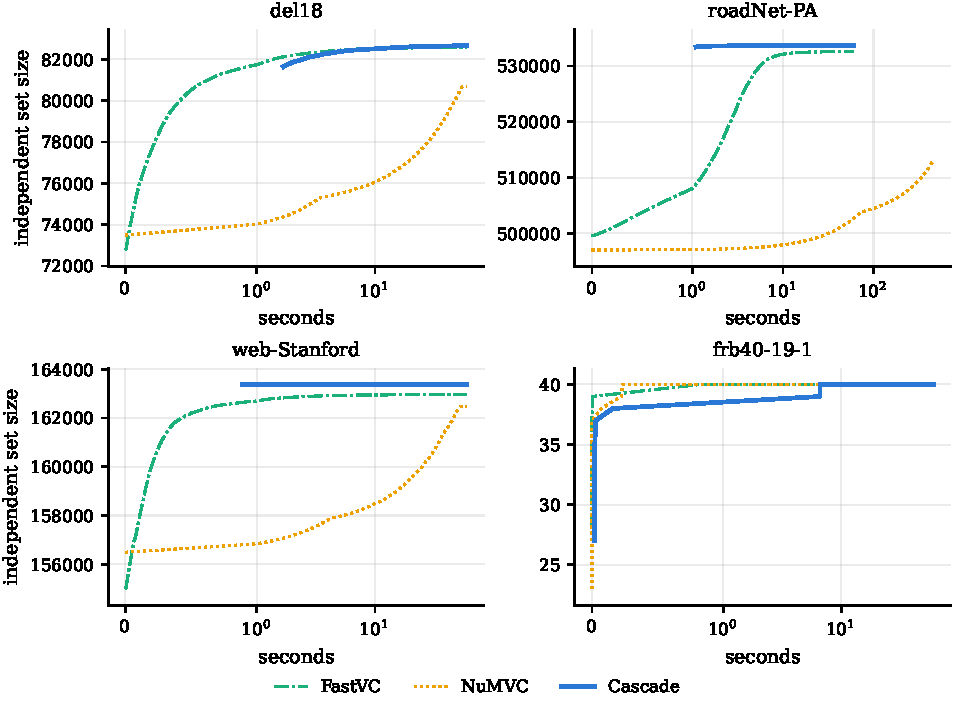
\includegraphics[width=\textwidth]{figures/convergence}
\caption{Incumbent size against wall-clock time at a 60-second budget, on a
symmetric-log time axis so the first second is legible. Note that the solvers
report at different granularities: ours records one point per search batch
(between 6 and 586 points here) while NuMVC and FastVC report every individual
improvement (up to 33\,000), so the apparent smoothness of a curve reflects how
often a solver reports, not how often it improves.}
\label{fig:convergence}
\end{figure}


\section{Exact solvers}
\label{sec:exact}

The method proposed here is a heuristic, and the question of how far its answers
sit from optimal is separate from how they compare with other heuristics. To
place them we ran three exact solvers and one integer-programming solver on the
instances small enough to admit them: the branch-and-reduce solver built from
our own components (\textsc{Cascade}-exact, the sub-solver of
Section~\ref{sec:implementation} applied to the whole graph), VCSolver
\citep{akiba2016}, the winner of the vertex cover track of PACE 2019
\citep{pace2019,hespe2020}, and HiGHS on the natural
integer program. Table~\ref{tab:exact} reports the results.

Three conclusions follow, and only the first is favourable to us. On the
instances that reduce almost completely --- \texttt{ca-AstroPh},
\texttt{ca-CondMat}, \texttt{email-Enron} --- all four prove optimality, and our
sub-solver is the fastest of them --- by a factor of 25 to 40 over HiGHS, three
to five over VCSolver, and a more modest 1.1 to 1.4 over the PACE portfolio ---
which is the property
the region move depends on: the sub-problems it generates are of exactly this
shape, and at $10^3$ to $10^4$ moves per second (Table~\ref{M-tab:regional}) they must each be solved in a fraction
of a millisecond.

Second, our exact solver is not competitive as an exact solver. On the BHOSLIB
family the PACE 2019 portfolio proves the optimum of \texttt{frb30-15-1},
\texttt{frb35-17-1} and \texttt{frb40-19-1} in under four seconds each, while
ours returns 25, 28 and 30 against the true 30, 35 and 40 and proves nothing.
It is built to be restarted millions of times on graphs of a few dozen vertices,
not to prove optimality on a dense graph of a thousand, and the table shows the
cost of that choice. Where a proof is wanted on instances of this kind, the
portfolio approach is the right tool.

Third, the integer-programming route is not a usable baseline at this scale, and
we record its failures rather than omitting it. HiGHS matches the optimum on the
three easy instances but exceeds the 60-second budget on most others, taking up
to 360\,s; on \texttt{frb45-21-1} through \texttt{frb53-24-1} it returns a single
vertex, on \texttt{rgg18} none at all, and on \texttt{del18} and
\texttt{web-Stanford} it emits no solution we could verify. On
\texttt{email-Enron} it reports optimality but the solution it writes has 22\,253
vertices against the 22\,255 that the other three solvers prove optimal and that
our verifier confirms; we therefore treat its optimality claims as unreliable
and its numbers as a lower bound on what a tuned commercial solver would do.
This is a statement about the formulation at this size, not about HiGHS: the
natural model has one variable per vertex and one constraint per edge, which for
the larger instances in the benchmark means tens of millions of constraints.

\begin{table}[htbp]
\centering
\small
\caption{Exact and integer-programming solvers under a 60-second budget, on the instances where any of them terminates. Each pair of columns gives the size returned and the wall-clock seconds; \textbf{bold} marks a value the solver proved optimal, and \textit{t/o} that it returned no solution within the budget. Higher is better for size, lower for time.}
\label{tab:exact}
\begin{tabular}{l l r r r r r r r r }
\toprule
& & \multicolumn{2}{c}{\textsc{Cascade}-exact} & \multicolumn{2}{c}{VCSolver} & \multicolumn{2}{c}{PACE 2019} & \multicolumn{2}{c}{HiGHS} \\
\cmidrule(lr){3-4}\cmidrule(lr){5-6}\cmidrule(lr){7-8}\cmidrule(lr){9-10}
Instance & Family & size & s & size & s & size & s & size & s \\
\midrule
\texttt{ca-AstroPh} & social & \textbf{6760} & 0.1 & \textbf{6760} & 0.3 & \textbf{6760} & 0.1 & \textbf{6760} & 4.0 \\
\texttt{ca-CondMat} & social & \textbf{9612} & 0.0 & \textbf{9612} & 0.2 & \textbf{9612} & 0.1 & \textbf{9612} & 1.3 \\
\texttt{email-Enron} & social & \textbf{22255} & 0.1 & \textbf{22255} & 0.4 & \textbf{22255} & 0.1 & \textbf{22253} & 2.0 \\
\texttt{del16} & geometric & 20474 & 60.1 & \textit{---} & \textit{t/o} & \textit{---} & \textit{t/o} & 9679 & 60.5 \\
\texttt{del18} & geometric & 73928 & 83.2 & \textit{---} & \textit{t/o} & \textit{---} & \textit{t/o} & \textit{---} & \textit{t/o} \\
\texttt{rgg16} & geometric & 16086 & 60.1 & \textbf{16086} & 0.7 & \textbf{16086} & 0.4 & 16086 & 60.6 \\
\texttt{rgg18} & geometric & 64271 & 60.3 & \textbf{64278} & 2.3 & \textbf{64278} & 2.2 & 0 & 240.8 \\
\texttt{web-Stanford} & web & 163376 & 60.6 & \textit{---} & \textit{t/o} & \textit{---} & \textit{t/o} & \textit{---} & \textit{t/o} \\
\texttt{frb30-15-1} & bhoslib & 25 & 60.0 & \textit{---} & \textit{t/o} & \textbf{30} & 1.8 & 28 & 60.1 \\
\texttt{frb35-17-1} & bhoslib & 28 & 60.0 & \textit{---} & \textit{t/o} & \textbf{35} & 2.5 & 30 & 60.2 \\
\texttt{frb40-19-1} & bhoslib & 30 & 60.0 & \textit{---} & \textit{t/o} & \textbf{40} & 3.6 & 2 & 60.2 \\
\texttt{frb45-21-1} & bhoslib & 34 & 60.1 & \textit{---} & \textit{t/o} & \textit{---} & \textit{t/o} & 1 & 60.2 \\
\texttt{frb50-23-1} & bhoslib & 35 & 60.1 & \textit{---} & \textit{t/o} & \textit{---} & \textit{t/o} & 1 & 60.2 \\
\texttt{frb53-24-1} & bhoslib & 37 & 60.0 & \textit{---} & \textit{t/o} & \textit{---} & \textit{t/o} & 1 & 60.8 \\
\texttt{frb59-26-1} & bhoslib & 42 & 60.1 & \textit{---} & \textit{t/o} & \textit{---} & \textit{t/o} & 30 & 60.3 \\
\bottomrule
\end{tabular}
\end{table}



\section{Replication on different hardware}
\label{sec:replication}

A computational study is only as convincing as its independence from the machine
it was run on. We therefore repeated the comparison on a second, unrelated
platform: virtual machines with two Intel Xeon cores at 2.20\,GHz and 12\,GB of
memory, against the four-core workstation used for the main tables. Every solver
was rebuilt from source on that platform by the provisioning script included
with our code, so nothing is carried over except the source.

Two properties of the replication are worth stating explicitly. First, all
solvers for a given instance were run on the same virtual machine, so each row
of the replication table is internally consistent; only different rows may come
from different machines, and those machines are of identical specification.
Splitting a single instance's solvers across machines would have made the
comparison meaningless, since the budget is a wall-clock budget and the amount
of work that fits into it depends on the processor. Second, the two largest
instances were excluded, because 12\,GB of memory is not enough for them; the
replication therefore covers 25 of the 27 instances.

Table~\ref{tab:replication} reports the outcome. The weak statement that
survives is that on each of the 25 instances the set of solvers attaining the
best value on the replication machine intersects the set attaining it on the
original machine. That statement alone does not say that the \emph{ranking} is
preserved, so we also compared every pair of the seven solvers on every
instance, 519 pairs in total with a value from both platforms. The sign of the
difference between the two solvers (better, equal, worse) is the same on both
platforms for 498 of them ($96.0\%$). In the remaining 21 the pair is equal on
one platform and strictly ordered on the other, and \emph{in none of the 519 does
the order reverse}. Restricted to \textsc{Cascade} against each baseline, 9 of
149 pairs change from equal to strict or back. The comparisons in
Main-text Section~
ef{M-sec:experiments} are therefore not artefacts of the machine to the
extent that two machines of this class can show.

The individual values move a little, and the table shows where. The two
deterministic solvers, reducing-peeling and near-linear kernelization, return
\emph{identical} values on all 25 instances, which is the control: it confirms that
the instances, the conversions and the verifier are the same on both platforms,
so any difference elsewhere comes from the solver rather than from the pipeline.
The five randomised solvers differ by a fraction of a percent on average, and
what difference there is concentrates on BHOSLIB, where the optima are small
enough that a one-vertex change is one to two percent. Away from that family our
own solver returns the same value on both machines on every road, web and social
instance, and differs by an average of $0.016\%$ on the geometric family.

Two caveats belong with this. The replication machine is slower, so a solver
that spends its whole budget does less work within it; that is visible as the
larger spreads for the vertex cover local search solvers, which have no
reduction phase to fall back on, and most sharply as NuMVC exceeding the cutoff
altogether on \texttt{roadNet-CA}, an instance it completed on the faster
machine. And a fixed wall-clock budget on two machines
of different speed is not the same experiment twice --- it is the same
\emph{protocol} twice, which is what a practitioner choosing a solver under a
deadline actually faces.

\begin{table}[htbp]
\centering
\small
\caption{Replication on a second platform. Each cell is the mean, over the instances of that family, of $100\,|s_2-s_1|/s_1$ where $s_1$ is the size the solver returned on the machine used for the main tables and $s_2$ the size it returned on the replication machine. LOWER IS BETTER: zero means the solver returned the same value on both machines. \emph{Same} counts the instances on which it did so exactly, over the instances where the solver returned a value on both machines; that denominator is 25 except for NuMVC, which exceeded the cutoff on \texttt{roadNet-CA} on the replication machine. \emph{Max} is the largest single relative difference.}
\label{tab:replication}
\fittable{
\begin{tabular}{l r r r r r r r}
\toprule
Solver & Geometric & Road & Web & Social & Bhoslib & Same & Max \\
\midrule
\textsc{Cascade} & 0.016 & 0.000 & 0.000 & 0.000 & 0.366 & 18/25 & 2.56 \\
ReduMIS & 0.124 & 0.000 & 0.000 & 0.000 & 0.000 & 22/25 & 0.74 \\
OnlineMIS & 0.608 & 0.113 & 0.157 & 0.000 & 0.000 & 16/25 & 1.76 \\
NuMVC & 0.021 & 0.006 & 0.008 & 0.002 & 0.560 & 8/24 & 2.00 \\
FastVC & 0.058 & 0.042 & 0.009 & 0.000 & 1.144 & 9/25 & 2.22 \\
NearLinear & 0.000 & 0.000 & 0.000 & 0.000 & 0.000 & 25/25 & 0.00 \\
LinearTime & 0.000 & 0.000 & 0.000 & 0.000 & 0.000 & 25/25 & 0.00 \\
\bottomrule
\end{tabular}
}
\end{table}



\section{Other parameters and time budgets}
Table~\ref{tab:sensitivity} varies four further parameters one at a time on three instances.
The comparison that makes the numbers interpretable is with the seed-to-seed spread
($0.024\%$ on the Delaunay family): a parameter whose range moves the answer by less than
that is not one the user needs to think about. \texttt{kernel\_share}, \texttt{lns\_start\_free}
and \texttt{lns\_slice} move \texttt{del18} by at most $0.013\%$ and \texttt{web-Stanford} by
at most $0.001\%$. \texttt{restart\_idle\_dives} is sensitive: $82\,592$ at 50, $82\,639$ at
100, $82\,659$ at the default 200, then $82\,655$ at both 400 and 800, so the safe direction
to err in is upwards. On the dense instance the spreads are $2.5$--$5\%$, within the seed
spread of that family, and one run per setting cannot separate a parameter effect from it.
\begin{table}[htbp]
\centering
\small
\caption{Parameter sensitivity. Each block varies one parameter over its range with the others held at their defaults; $\star$ marks the default. Cells are the size returned at a 60-second budget, HIGHER IS BETTER. The \emph{spread} line under each block is $100\,(\max-\min)/\max$ over that block, per instance, to be read against the seed-to-seed spread of Section~\ref{M-sec:experiments}: $0.024\%$ on the geometric family and up to $2.5\%$ on BHOSLIB.}
\label{tab:sensitivity}
\fittable{
\begin{tabular}{l r r r r }
\toprule
Parameter & Value & \texttt{del18} & \texttt{frb40-19-1} & \texttt{web-Stanford} \\
\midrule
\texttt{kernel\_share} & 0.1 & 82656 & 39 & 163375 \\
 & 0.2 & 82655 & 39 & 163375 \\
 & 0.3$\star$ & 82655 & 40 & 163375 \\
 & 0.5 & 82656 & 40 & 163375 \\
 & 0.7 & 82655 & 39 & 163375 \\
\cmidrule(lr){3-5}
& \emph{spread \%} & \emph{0.001} & \emph{2.500} & \emph{0.000} \\\\
\midrule
\texttt{lns\_start\_free} & 1 & 82648 & 39 & 163374 \\
 & 2 & 82650 & 39 & 163375 \\
 & 4$\star$ & 82655 & 39 & 163375 \\
 & 8 & 82650 & 40 & 163376 \\
 & 16 & 82659 & 38 & 163374 \\
\cmidrule(lr){3-5}
& \emph{spread \%} & \emph{0.013} & \emph{5.000} & \emph{0.001} \\\\
\midrule
\texttt{lns\_slice} & 0.01 & 82651 & 39 & 163375 \\
 & 0.02 & 82649 & 40 & 163375 \\
 & 0.05$\star$ & 82656 & 39 & 163375 \\
 & 0.1 & 82656 & 39 & 163375 \\
 & 0.2 & 82656 & 39 & 163375 \\
\cmidrule(lr){3-5}
& \emph{spread \%} & \emph{0.008} & \emph{2.500} & \emph{0.000} \\\\
\midrule
\texttt{restart\_idle\_dives} & 50 & 82592 & 39 & 163373 \\
 & 100 & 82639 & 39 & 163375 \\
 & 200$\star$ & 82659 & 40 & 163375 \\
 & 400 & 82655 & 39 & 163375 \\
 & 800 & 82655 & 40 & 163375 \\
\cmidrule(lr){3-5}
& \emph{spread \%} & \emph{0.081} & \emph{2.500} & \emph{0.001} \\\\
\bottomrule
\end{tabular}
}
\end{table}

Table~\ref{tab:budget} gives the wall-clock time actually taken under the 60\,s budget.
\begin{table}[htbp]
\centering
\caption{Wall-clock time actually taken under a 60\,s budget, over all instances. Time is measured around the whole process, so it includes reading and any construction phase.}
\label{tab:budget}
\begin{tabular}{lrrrr}
\toprule
Algorithm & median & mean & max & runs $>1.5\times$ budget \\
\midrule
\textsc{Cascade} & 60.1 & 48.3 & 75.0 & 0 \\
ReduMIS & 60.2 & 69.7 & 660.2 & 2 \\
OnlineMIS & 60.0 & 44.0 & 66.8 & 0 \\
NearLinear & 0.2 & 1.1 & 15.4 & 0 \\
LinearTime & 0.1 & 0.3 & 2.5 & 0 \\
NuMVC & 85.9 & 204.3 & 960.0 & 12 \\
FastVC & 60.2 & 60.7 & 67.5 & 0 \\
\bottomrule
\end{tabular}
\end{table}


\section{Implementation notes}

\label{sec:implementation}

Reductions and branching decisions both mutate the graph and must be reversible,
at every node of the sub-searches and after every region move. We use a compressed
adjacency array in which each entry stores the position of its twin, together
with a per-vertex pointer separating the live neighbours from the dead ones.
Deleting a vertex $v$ swaps its entry to the end of each live neighbour's range
and decrements that neighbour's pointer; undoing the deletion merely increments
the pointers again. Nothing has to be swapped back, because no later operation
touches an entry outside the live range. Both directions cost $O(\deg v)$ and
carry no payload, and degrees remain exact throughout.

Degree-2 folding introduces edges that do not fit in the static array; these go
into per-vertex overflow lists which are append-only and undone by a pop, and
which are allocated only for vertices that actually take part in a fold.

Two engineering details matter for throughput. First, each node of a sub-search
owns an exact list of its live vertices, built by filtering its parent's. An
earlier version shared one list and could drop a vertex when a fold created a new
one; the clique-cover bound then failed to cover that vertex, came out too small,
and pruned optimal solutions while still reporting that optimality had been
proven. Second, the sub-solver is reused across region moves instead of being
constructed afresh, since at a hundred thousand moves per minute the set-up of
the graph and reduction state costs more than the search itself.

To give these choices a number, the full configuration in the ablation runs of
Main-text Section~
ef{M-sec:regional} (three seeds, three processes sharing the machine)
kernelizes \texttt{del18}, 262\,144 vertices, in $1.6$--$2.0$\,s, completes the
first dive in a further $0.55$--$0.63$\,s and performs $102\,906$--$112\,414$
region moves in the rest of the 60\,s, one every $560\,\mu$s on average. On
\texttt{web-Stanford} the figures are $1.0$--$1.1$\,s, $0.03$--$0.05$\,s and
$70\,496$--$91\,130$ moves. Those rates are what the reuse of the sub-solver and
the payload-free undo buy; the throughput, not the asymptotics, is what makes
an exactly-solved neighbourhood practical.

The reduction queue is seeded in increasing order of degree, so that the cheap
rules fire on the vertices most likely to trigger cascades before any expensive
test is attempted on a hub. This is a design choice, not a measured result of
this paper: we did not keep a plain-order variant and report no comparison.

The last of these details is the one that decides whether the solver keeps its
promise at all. Kernelization is run to exhaustion in principle, but on some
graphs exhaustion is unaffordable: on \texttt{soc-pokec}, 1.6 million vertices,
running the rules to a fixed point takes $180.5$\,s in an early measurement on
the main-table machine and $332$\,s in the loaded measurement of
Table~\ref{M-tab:kernels}, three or more times the entire 60-second budget, so a
solver that insisted on finishing would return nothing at all. We therefore give kernelization a fixed share of the budget --- $0.3$ by
default --- and stop it where it stands when that share is spent, keeping
whatever reductions have been applied and continuing with the rest. On
\texttt{soc-pokec} the phase is cut off at $18.0$\,s, exactly the share, and the
solver returns 788\,868 within its budget. The truncation is recorded in the
run records, so a reader can see on which instances the kernel is partial.
This is the difference between a method that respects a deadline and one that
merely has a time limit in its interface.

Correctness is checked by comparing the exact solver against exhaustive search on
random graphs, repeating the comparison with each reduction rule disabled in
turn, and by verifying that every solution our solver reports is independent and maximal.


\begin{figure}[htbp]
\centering
\resizebox{\textwidth}{!}{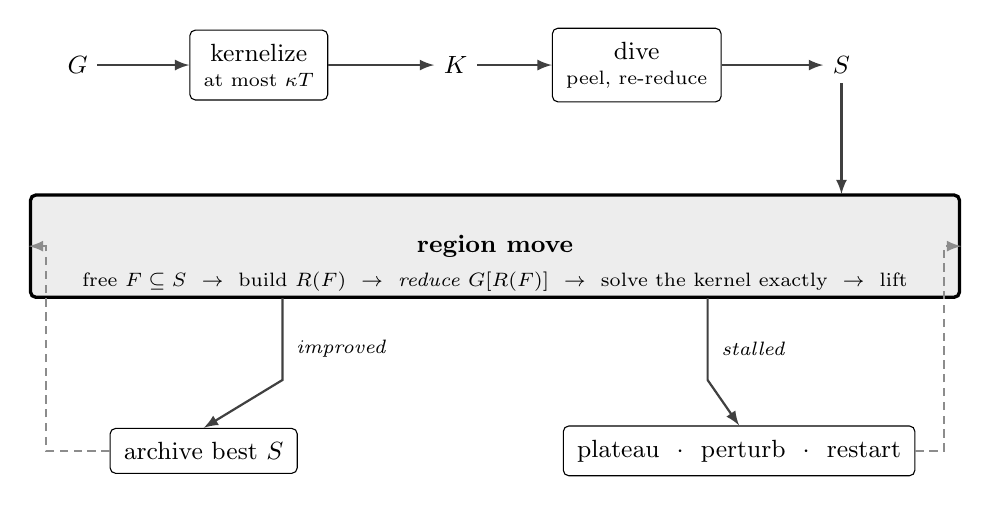
\begin{tikzpicture}[
  font=\small,
  box/.style={draw, rounded corners=2pt, align=center, inner sep=5pt, fill=white},
  core/.style={box, very thick, fill=black!7},
  flow/.style={draw, -latex, black!75, thick},
  back/.style={draw, -latex, black!45, thick, densely dashed},
  lbl/.style={font=\scriptsize\itshape, inner sep=2pt},
]

% ---------------- once, before the search ----------------
\node          (g)    at ( 0.0, 0) {$G$};
\node[box]     (kern) at ( 2.3, 0) {kernelize\\[-2pt]{\scriptsize at most $\kappa T$}};
\node          (k)    at ( 4.8, 0) {$K$};
\node[box]     (dive) at ( 7.1, 0) {dive\\[-2pt]{\scriptsize peel, re-reduce}};
\node          (s)    at ( 9.7, 0) {$S$};

\draw[flow] (g)    -- (kern);
\draw[flow] (kern) -- (k);
\draw[flow] (k)    -- (dive);
\draw[flow] (dive) -- (s);

% ---------------- the repeated part ----------------
\node[core, minimum width=118mm, minimum height=13mm] (move) at (5.3,-2.3)
  {\textbf{region move}};
\node[align=center] at (5.3,-2.75)
  {\scriptsize free $F\subseteq S$ \ $\rightarrow$ \ build $R(F)$ \ $\rightarrow$ \
   \emph{reduce $G[R(F)]$} \ $\rightarrow$ \ solve the kernel exactly \ $\rightarrow$ \ lift};

\node[box] (archive) at (1.6,-4.9) {archive best $S$};
\node[box] (escape)  at (8.4,-4.9) {plateau \ $\cdot$ \ perturb \ $\cdot$ \ restart};

% incumbent enters the loop
\draw[flow] (s) -- (9.7,-1.0) -- (9.7,-1.64);

% and the loop leaves it two ways
\draw[flow] (2.6,-2.96) -- (2.6,-4.0) -- (archive.north);
\node[lbl, anchor=west] at (2.7,-3.6) {improved};
\draw[flow] (8.0,-2.96) -- (8.0,-4.0) -- (escape.north);
\node[lbl, anchor=west] at (8.1,-3.6) {stalled};

% both paths return to the move
\draw[back] (archive.west) -- (-0.4,-4.9) -- (-0.4,-2.3) -- (move.west);
\draw[back] (escape.east)  -- (11.0,-4.9) -- (11.0,-2.3) -- (move.east);

\end{tikzpicture}
}
\caption{Where the work goes. Kernelization and the dive run once, the first of
them bounded by a share $\kappa$ of the budget so that it cannot consume the
whole of it; everything after that is region moves. The
step set in italics is what distinguishes the method: the reduction rules are
applied \emph{inside} each move, to the region rather than to the input, which is
what makes solving the region exactly affordable. A move never returns a worse
solution than it received, so the only reason to leave the loop is that it has
stopped improving, and the escape mechanisms exist to put it back.}
\label{fig:pipeline}
\end{figure}
\section{Instance provenance}
\label{app:provenance}

Table~\ref{tab:provenance} records where each instance came from, so that the
benchmark set can be rebuilt exactly. Three points deserve emphasis, because each
is a way in which two studies can report different numbers for what they believe
is the same graph.

First, the real-world instances are distributed as directed or multiply-listed
edge lists. We read every file as undirected, discard self-loops and duplicate
edges, and renumber the vertices consecutively; the $n$ and $m$ in the table are
the values after this normalisation, and they are what our solver and every
baseline receive. Isolated vertices are retained rather than dropped. Removing $q$ isolated
vertices lowers the independence number by exactly $q$, so a study that drops
them reports values smaller by $q$ than one that keeps them, and the two are not
comparable unless $q$ is stated.

Second, the BHOSLIB instances are published in two forms, and the distinction is
easy to miss. The Network Repository archive ships the \emph{clique} form, whose
independence number is the size of a Model-RB domain rather than the advertised
$\alpha$: on \texttt{frb30-15-1} that form has 83\,198 edges and every solver we
tried returned exactly 15. The form used here, and the one the published
$\alpha$ values refer to, is its complement, with 17\,827 edges and $\alpha=30$.
Our converter takes the complement explicitly. A study that omits this step is
not solving a hard instance at all, and its BHOSLIB numbers cannot be compared
with anyone else's.

Third, the geometric instances are generated rather than downloaded. They come
from \texttt{tools/gen\_instances.py} at seed 1: the Delaunay instances are the
Delaunay triangulation of $2^{k}$ uniform points in the unit square, and the
random geometric instances connect points within the radius that gives an
expected average degree of 8. The generator is deterministic given the seed, so
the instances in the table are reproducible, but they are \emph{not} the DIMACS
implementation-challenge graphs of the same names, and the two should not be
compared.

\footnotesize
\setlength{\tabcolsep}{3pt}
\begin{longtable}{l l r r r r l}
\caption{Provenance and basic statistics of the 27 benchmark instances. $\bar{d}$ is the average degree and $\Delta$ the maximum degree. Sources: SNAP is \texttt{snap.stanford.edu/data}, where each instance is the file of its own name (the \texttt{com-*} graphs are the \texttt{.ungraph} files under \texttt{bigdata/communities}); $^{\dagger}$ Network Repository \texttt{bhoslib}, used in complement as Section~\ref{sec:experiments} explains; $^{\ddagger}$ produced by \texttt{tools/gen\_instances.py} at seed 1.}\label{tab:provenance}\\
\toprule
Instance & Family & $n$ & $m$ & $\bar{d}$ & $\Delta$ & Source \\
\midrule
\endfirsthead
\multicolumn{7}{l}{\itshape Table~\ref{tab:provenance}, continued}\\
\toprule
Instance & Family & $n$ & $m$ & $\bar{d}$ & $\Delta$ & Source \\
\midrule
\endhead
\midrule \multicolumn{7}{r}{\itshape continued on next page}\\
\endfoot
\bottomrule
\endlastfoot
\texttt{rgg16} & geometric & 65,501 & 260,438 & 8.0 & 24 & generated$^{\ddagger}$ \\
\texttt{del16} & geometric & 65,536 & 196,583 & 6.0 & 20 & generated$^{\ddagger}$ \\
\texttt{rgg18} & geometric & 262,011 & 1,046,301 & 8.0 & 23 & generated$^{\ddagger}$ \\
\texttt{del18} & geometric & 262,144 & 786,401 & 6.0 & 21 & generated$^{\ddagger}$ \\
\texttt{rgg20} & geometric & 1,048,171 & 4,188,702 & 8.0 & 24 & generated$^{\ddagger}$ \\
\texttt{del20} & geometric & 1,048,576 & 3,145,692 & 6.0 & 22 & generated$^{\ddagger}$ \\
\texttt{roadNet-PA} & road & 1,088,092 & 1,541,898 & 2.8 & 9 & SNAP \\
\texttt{roadNet-CA} & road & 1,965,206 & 2,766,607 & 2.8 & 12 & SNAP \\
\texttt{web-Stanford} & web & 281,903 & 1,992,636 & 14.1 & 38,625 & SNAP \\
\texttt{web-BerkStan} & web & 685,230 & 6,649,470 & 19.4 & 84,230 & SNAP \\
\texttt{ca-AstroPh} & social & 18,772 & 198,050 & 21.1 & 504 & SNAP \\
\texttt{ca-CondMat} & social & 23,133 & 93,439 & 8.1 & 279 & SNAP \\
\texttt{email-Enron} & social & 36,692 & 183,831 & 10.0 & 1,383 & SNAP \\
\texttt{com-dblp} & social & 317,080 & 1,049,866 & 6.6 & 343 & SNAP \\
\texttt{com-amazon} & social & 334,863 & 925,872 & 5.5 & 549 & SNAP \\
\texttt{com-youtube} & social & 1,134,890 & 2,987,624 & 5.3 & 28,754 & SNAP \\
\texttt{soc-pokec-relationships} & social & 1,632,803 & 22,301,964 & 27.3 & 14,854 & SNAP \\
\texttt{as-skitter} & social & 1,696,415 & 11,095,298 & 13.1 & 35,455 & SNAP \\
\texttt{wiki-Talk} & social & 2,394,385 & 4,659,565 & 3.9 & 100,029 & SNAP \\
\texttt{com-lj} & social & 3,997,962 & 34,681,189 & 17.3 & 14,815 & SNAP \\
\texttt{frb30-15-1} & bhoslib & 450 & 17,827 & 79.2 & 122 & NetRep$^{\dagger}$ \\
\texttt{frb35-17-1} & bhoslib & 595 & 27,856 & 93.6 & 132 & NetRep$^{\dagger}$ \\
\texttt{frb40-19-1} & bhoslib & 760 & 41,314 & 108.7 & 178 & NetRep$^{\dagger}$ \\
\texttt{frb45-21-1} & bhoslib & 945 & 59,186 & 125.3 & 188 & NetRep$^{\dagger}$ \\
\texttt{frb50-23-1} & bhoslib & 1,150 & 80,072 & 139.3 & 208 & NetRep$^{\dagger}$ \\
\texttt{frb53-24-1} & bhoslib & 1,272 & 94,227 & 148.2 & 232 & NetRep$^{\dagger}$ \\
\texttt{frb59-26-1} & bhoslib & 1,534 & 126,555 & 165.0 & 277 & NetRep$^{\dagger}$ \\
\end{longtable}
\setlength{\tabcolsep}{6pt}
\normalsize


\setcounter{table}{0}
\section{Complete per-instance results}
\label{app:full}

Table~\ref{tab:appendix} lists every run behind the summary tables, so that the
aggregates can be checked against the individual measurements. The raw records,
including the seed study and the replication, are distributed with the source.

\begin{longtable}{llrr rr}
\caption{Complete per-instance results at the 60\,s budget: size found and wall-clock seconds. A dash means the solver returned no solution within the cutoff.}\label{tab:appendix}\\
\toprule
Instance & Solver & $n$ & $m$ & size & seconds \\
\midrule
\endfirsthead
\toprule Instance & Solver & $n$ & $m$ & size & seconds \\ \midrule \endhead
\bottomrule \endfoot
\texttt{rgg16} & \textsc{Cascade} & 65,501 & 260,438 & 16086 & 60.1 \\
 & ReduMIS &  &  & 16086 & 9.5 \\
 & OnlineMIS &  &  & 16082 & 60.1 \\
 & NuMVC &  &  & 15905 & 60.3 \\
 & FastVC &  &  & 16085 & 60.0 \\
 & NearLinear &  &  & 16035 & 0.1 \\
 & LinearTime &  &  & 15321 & 0.0 \\
\addlinespace
\texttt{del16} & \textsc{Cascade} & 65,536 & 196,583 & 20647 & 60.1 \\
 & ReduMIS &  &  & 20640 & 60.2 \\
 & OnlineMIS &  &  & 20630 & 60.1 \\
 & NuMVC &  &  & 20180 & 60.3 \\
 & FastVC &  &  & 20638 & 60.0 \\
 & NearLinear &  &  & 20284 & 0.1 \\
 & LinearTime &  &  & 20213 & 0.0 \\
\addlinespace
\texttt{rgg18} & \textsc{Cascade} & 262,011 & 1,046,301 & 64278 & 60.3 \\
 & ReduMIS &  &  & 64278 & 12.6 \\
 & OnlineMIS &  &  & 63912 & 60.5 \\
 & NuMVC &  &  & 62548 & 87.2 \\
 & FastVC &  &  & 64242 & 60.2 \\
 & NearLinear &  &  & 64094 & 0.3 \\
 & LinearTime &  &  & 61282 & 0.1 \\
\addlinespace
\texttt{del18} & \textsc{Cascade} & 262,144 & 786,401 & 82656 & 60.2 \\
 & ReduMIS &  &  & 82385 & 60.7 \\
 & OnlineMIS &  &  & 82019 & 60.4 \\
 & NuMVC &  &  & 80695 & 120.7 \\
 & FastVC &  &  & 82579 & 60.1 \\
 & NearLinear &  &  & 81211 & 0.7 \\
 & LinearTime &  &  & 80881 & 0.1 \\
\addlinespace
\texttt{rgg20} & \textsc{Cascade} & 1,048,171 & 4,188,702 & 256994 & 61.3 \\
 & ReduMIS &  &  & 256994 & 23.4 \\
 & OnlineMIS &  &  & 242366 & 61.7 \\
 & NuMVC &  &  & 239118 & 490.2 \\
 & FastVC &  &  & 256680 & 60.8 \\
 & NearLinear &  &  & 256277 & 1.8 \\
 & LinearTime &  &  & 244769 & 0.5 \\
\addlinespace
\texttt{del20} & \textsc{Cascade} & 1,048,576 & 3,145,692 & 330066 & 61.1 \\
 & ReduMIS &  &  & 321566 & 258.2 \\
 & OnlineMIS &  &  & 311146 & 61.7 \\
 & NuMVC &  &  & 311421 & 428.9 \\
 & FastVC &  &  & 329802 & 60.6 \\
 & NearLinear &  &  & 324619 & 4.7 \\
 & LinearTime &  &  & 323438 & 0.4 \\
\addlinespace
\texttt{roadNet-PA} & \textsc{Cascade} & 1,088,092 & 1,541,898 & 533627 & 60.8 \\
 & ReduMIS &  &  & 533628 & 37.2 \\
 & OnlineMIS &  &  & 515876 & 61.2 \\
 & NuMVC &  &  & 513067 & 451.1 \\
 & FastVC &  &  & 532571 & 60.3 \\
 & NearLinear &  &  & 531184 & 0.6 \\
 & LinearTime &  &  & 530910 & 0.1 \\
\addlinespace
\texttt{roadNet-CA} & \textsc{Cascade} & 1,965,206 & 2,766,607 & 961851 & 61.5 \\
 & ReduMIS &  &  & 961851 & 62.1 \\
 & OnlineMIS &  &  & 924236 & 62.2 \\
 & NuMVC &  &  & 915797 & 911.9 \\
 & FastVC &  &  & 959909 & 60.6 \\
 & NearLinear &  &  & 957199 & 1.8 \\
 & LinearTime &  &  & 956573 & 0.3 \\
\addlinespace
\texttt{ca-AstroPh} & \textsc{Cascade} & 18,772 & 198,050 & 6760 & 0.1 \\
 & ReduMIS &  &  & 6760 & 0.2 \\
 & OnlineMIS &  &  & 6760 & 60.1 \\
 & NuMVC &  &  & 6760 & 61.3 \\
 & FastVC &  &  & 6760 & 60.0 \\
 & NearLinear &  &  & 6760 & 0.0 \\
 & LinearTime &  &  & 6759 & 0.0 \\
\addlinespace
\texttt{ca-CondMat} & \textsc{Cascade} & 23,133 & 93,439 & 9612 & 0.1 \\
 & ReduMIS &  &  & 9612 & 0.1 \\
 & OnlineMIS &  &  & 9601 & 0.0 \\
 & NuMVC &  &  & 9611 & 60.5 \\
 & FastVC &  &  & 9612 & 60.0 \\
 & NearLinear &  &  & 9612 & 0.0 \\
 & LinearTime &  &  & 9611 & 0.0 \\
\addlinespace
\texttt{email-Enron} & \textsc{Cascade} & 36,692 & 183,831 & 22255 & 0.1 \\
 & ReduMIS &  &  & 22255 & 0.2 \\
 & OnlineMIS &  &  & 22227 & 0.1 \\
 & NuMVC &  &  & 22253 & 60.2 \\
 & FastVC &  &  & 22255 & 60.0 \\
 & NearLinear &  &  & 22255 & 0.0 \\
 & LinearTime &  &  & 22255 & 0.0 \\
\addlinespace
\texttt{com-dblp} & \textsc{Cascade} & 317,080 & 1,049,866 & 152131 & 0.4 \\
 & ReduMIS &  &  & 152131 & 0.6 \\
 & OnlineMIS &  &  & 152061 & 0.6 \\
 & NuMVC &  &  & 152112 & 85.9 \\
 & FastVC &  &  & 152131 & 60.2 \\
 & NearLinear &  &  & 152131 & 0.1 \\
 & LinearTime &  &  & 152129 & 0.1 \\
\addlinespace
\texttt{com-amazon} & \textsc{Cascade} & 334,863 & 925,872 & 174632 & 60.3 \\
 & ReduMIS &  &  & 174632 & 10.1 \\
 & OnlineMIS &  &  & 172685 & 0.6 \\
 & NuMVC &  &  & 174510 & 114.1 \\
 & FastVC &  &  & 174605 & 60.2 \\
 & NearLinear &  &  & 174627 & 0.1 \\
 & LinearTime &  &  & 174612 & 0.1 \\
\addlinespace
\texttt{com-youtube} & \textsc{Cascade} & 1,134,890 & 2,987,624 & 857945 & 1.3 \\
 & ReduMIS &  &  & 857945 & 1.8 \\
 & OnlineMIS &  &  & 857680 & 1.7 \\
 & NuMVC &  &  & 857708 & 143.2 \\
 & FastVC &  &  & 857945 & 60.6 \\
 & NearLinear &  &  & 857945 & 0.2 \\
 & LinearTime &  &  & 857944 & 0.2 \\
\addlinespace
\texttt{soc-pokec-relationships} & \textsc{Cascade} & 1,632,803 & 22,301,964 & 788866 & 72.9 \\
 & ReduMIS &  &  & -- & 660.2 \\
 & OnlineMIS &  &  & 776663 & 66.8 \\
 & NuMVC &  &  & 787320 & 444.4 \\
 & FastVC &  &  & 789352 & 64.0 \\
 & NearLinear &  &  & 789161 & 15.4 \\
 & LinearTime &  &  & 789003 & 1.6 \\
\addlinespace
\texttt{as-skitter} & \textsc{Cascade} & 1,696,415 & 11,095,298 & 1170576 & 64.5 \\
 & ReduMIS &  &  & 1170580 & 64.7 \\
 & OnlineMIS &  &  & 1152300 & 6.3 \\
 & NuMVC &  &  & 1168352 & 266.2 \\
 & FastVC &  &  & 1168417 & 61.9 \\
 & NearLinear &  &  & 1170541 & 0.7 \\
 & LinearTime &  &  & 1170410 & 0.5 \\
\addlinespace
\texttt{wiki-Talk} & \textsc{Cascade} & 2,394,385 & 4,659,565 & 2338222 & 2.5 \\
 & ReduMIS &  &  & 2338222 & 34.0 \\
 & OnlineMIS &  &  & 2338207 & 3.1 \\
 & NuMVC &  &  & 2338220 & 66.0 \\
 & FastVC &  &  & 2338222 & 61.1 \\
 & NearLinear &  &  & 2338222 & 0.3 \\
 & LinearTime &  &  & 2338222 & 0.3 \\
\addlinespace
\texttt{com-lj} & \textsc{Cascade} & 3,997,962 & 34,681,189 & 2085626 & 75.0 \\
 & ReduMIS &  &  & 2085626 & 68.8 \\
 & OnlineMIS &  &  & 2066610 & 16.9 \\
 & NuMVC &  &  & -- & 960.0 \\
 & FastVC &  &  & 2085169 & 67.5 \\
 & NearLinear &  &  & 2085604 & 2.2 \\
 & LinearTime &  &  & 2085353 & 2.5 \\
\addlinespace
\texttt{web-Stanford} & \textsc{Cascade} & 281,903 & 1,992,636 & 163375 & 60.7 \\
 & ReduMIS &  &  & 163390 & 31.3 \\
 & OnlineMIS &  &  & 162453 & 60.7 \\
 & NuMVC &  &  & 162453 & 92.3 \\
 & FastVC &  &  & 162953 & 60.3 \\
 & NearLinear &  &  & 163198 & 0.3 \\
 & LinearTime &  &  & 163121 & 0.1 \\
\addlinespace
\texttt{web-BerkStan} & \textsc{Cascade} & 685,230 & 6,649,470 & 408380 & 61.7 \\
 & ReduMIS &  &  & 408482 & 59.8 \\
 & OnlineMIS &  &  & 406062 & 61.9 \\
 & NuMVC &  &  & 405003 & 131.2 \\
 & FastVC &  &  & 406323 & 60.9 \\
 & NearLinear &  &  & 408054 & 0.7 \\
 & LinearTime &  &  & 407716 & 0.2 \\
\addlinespace
\texttt{frb30-15-1} & \textsc{Cascade} & 450 & 17,827 & 30 & 60.0 \\
 & ReduMIS &  &  & 30 & 60.4 \\
 & OnlineMIS &  &  & 29 & 60.0 \\
 & NuMVC &  &  & 30 & 60.0 \\
 & FastVC &  &  & 30 & 60.0 \\
 & NearLinear &  &  & 24 & 0.0 \\
 & LinearTime &  &  & 22 & 0.0 \\
\addlinespace
\texttt{frb35-17-1} & \textsc{Cascade} & 595 & 27,856 & 34 & 60.0 \\
 & ReduMIS &  &  & 35 & 60.5 \\
 & OnlineMIS &  &  & 33 & 60.0 \\
 & NuMVC &  &  & 35 & 60.0 \\
 & FastVC &  &  & 35 & 60.0 \\
 & NearLinear &  &  & 27 & 0.0 \\
 & LinearTime &  &  & 25 & 0.0 \\
\addlinespace
\texttt{frb40-19-1} & \textsc{Cascade} & 760 & 41,314 & 39 & 60.0 \\
 & ReduMIS &  &  & 40 & 61.2 \\
 & OnlineMIS &  &  & 39 & 60.0 \\
 & NuMVC &  &  & 40 & 60.0 \\
 & FastVC &  &  & 40 & 60.0 \\
 & NearLinear &  &  & 27 & 0.1 \\
 & LinearTime &  &  & 29 & 0.0 \\
\addlinespace
\texttt{frb45-21-1} & \textsc{Cascade} & 945 & 59,186 & 43 & 60.0 \\
 & ReduMIS &  &  & 43 & 60.6 \\
 & OnlineMIS &  &  & 42 & 60.0 \\
 & NuMVC &  &  & 45 & 60.1 \\
 & FastVC &  &  & 45 & 60.0 \\
 & NearLinear &  &  & 33 & 0.1 \\
 & LinearTime &  &  & 32 & 0.0 \\
\addlinespace
\texttt{frb50-23-1} & \textsc{Cascade} & 1,150 & 80,072 & 48 & 60.0 \\
 & ReduMIS &  &  & 49 & 61.1 \\
 & OnlineMIS &  &  & 48 & 60.0 \\
 & NuMVC &  &  & 50 & 60.1 \\
 & FastVC &  &  & 49 & 60.0 \\
 & NearLinear &  &  & 35 & 0.1 \\
 & LinearTime &  &  & 33 & 0.0 \\
\addlinespace
\texttt{frb53-24-1} & \textsc{Cascade} & 1,272 & 94,227 & 50 & 60.0 \\
 & ReduMIS &  &  & 51 & 60.6 \\
 & OnlineMIS &  &  & 49 & 60.0 \\
 & NuMVC &  &  & 52 & 60.1 \\
 & FastVC &  &  & 51 & 60.0 \\
 & NearLinear &  &  & 38 & 0.2 \\
 & LinearTime &  &  & 40 & 0.0 \\
\addlinespace
\texttt{frb59-26-1} & \textsc{Cascade} & 1,534 & 126,555 & 56 & 60.0 \\
 & ReduMIS &  &  & 57 & 62.1 \\
 & OnlineMIS &  &  & 56 & 60.0 \\
 & NuMVC &  &  & 58 & 60.2 \\
 & FastVC &  &  & 56 & 60.0 \\
 & NearLinear &  &  & 43 & 0.2 \\
 & LinearTime &  &  & 43 & 0.0 \\
\addlinespace
\end{longtable}



\bibliographystyle{elsarticle-harv}
\bibliography{refs}
\end{document}
